% Template for ICASSP-2016 paper; to be used with:
%          spconf.sty  - ICASSP/ICIP LaTeX style file, and
%          IEEEbib.bst - IEEE bibliography style file.
% --------------------------------------------------------------------------
\documentclass{article}
\usepackage{spconf,amsmath,graphicx}
\usepackage{blindtext}
\usepackage[utf8]{inputenc}
\usepackage{hyperref}

% Example definitions.
% --------------------
\def\x{{\mathbf x}}
\def\L{{\cal L}}

% Title.
% ------
\title{AUTOMATED TRANSCRIPTION OF DRUMSOUNDS}
%
% Single address.
% ---------------
\name{Anyere Bendrien, Maximilian Wagenbach
    \thanks{Thanks to Holger Kirchhof and Tim Flohrer for assistance. Also thanks to TELECOM ParisTech - Dep. TSIe for generously providing the ENST drum test data set.}}
\address{Technical University of Berlin\\
    Audiocommunication Group\\
    Einsteinufer 17, 10587 Berlin}
%
% For example:
% ------------
%\address{School\\
%	Department\\
%	Address}
%
% Two addresses (uncomment and modify for two-address case).
% ----------------------------------------------------------
%\twoauthors
%  {A. Author-one, B. Author-two\sthanks{Thanks to XYZ agency for funding.}}
%	{School A-B\\
%	Department A-B\\
%	Address A-B}
%  {C. Author-three, D. Author-four\sthanks{The fourth author performed the work
%	while at ...}}
%	{School C-D\\
%	Department C-D\\
%	Address C-D}
%
\begin{document}
%\ninept
%
\maketitle
%
\begin{abstract}
Using math to do magic is easy.
While it is very easy for us humans to find patterns and percussive events in music such a task is very difficult for a computer.
In this research we showed that it is possible for a computer to find the exact time points of drum events in a piece of music by using non-negative matrix factorization.
Generating such a so called drum transcription can have lots of different applications.
By using relatively straightforward math and well established techniques that others before us have researched we hoped to get a reliable drum transcription algorithm.
In doing so we were able to get detection rates of up to 90\%.

%Stark verkürzte, überblicksartige Darstellung von Forschungsbedarf, Fragestellung, Methode, erwartetem Ergebnis und Nutzen.
%The abstract should contain about 100 to 150 words.
\end{abstract}
%
\begin{keywords}
Drum Transcription, Non-Negative Matrix Factorization, Onset Detection%, Profit
\end{keywords}
%
\section{Introduction}
\label{sec:intro}

For this research paper we looked into the topic of generating a drum transcription from a piece of music containing a recording of a drum kit.
Drum transcription is considered a classical music information retrieval (MIR) problem, where you want to extract information from a mixed piece of music.
In order to achieve this an algorithm is applied to the raw sound data to find the time points where a drum event happens in the song.
This list of time points and a corresponding flag with the kind of the drum event is called the drum transcription. 
While in theory this can be used to find any kind of event within a musical piece, we focused mainly on basic drum sounds in our research.

The transcription of the drum track of a song can be useful in many cases.
The simplest would be to generate the sheet music for a song where the original has been lost or is not available.
It can also be used for more sophisticated use cases like a conversion of a audio file to a MIDI sequence (known as Audio-to-MIDI).
For syncing visuals to music in VJing or light show applications (Sound-to-Light) a drum transcription is also an integral part.
Furthermore the drum transcription of a song can be used as a basis for more complicated MIR analysis.
For example using the results of the drum transcription a Beats per Minute (BPM) detection can be build, which in turn can then be the basis of a tempo detection algorithm.
Overall the drum transcription of a song is a basic but versatile information, that can be used in many different applications.


On first sight extracting the time point of a drum hit for a polyphonic, mixed piece of music sounds like a difficult task.
In fact though there are multiple mathematically simple algorithm to achieve that.
For this research we took an algorithm commonly used for these kind of problems: the non-negative matrix factorization (NMF).
Section \ref{sec:algo} will show a detailed explanation of how the NMF works.


\noindent\makebox[\linewidth]{\rule{\linewidth}{0.4pt}}
context, problem, use cases
definitions
paper overview

%Kurzes Umreißen des Themengebiets mit schneller Fokussierung auf den zu untersuchenden Gegenstand.
%Hierzu können technikhistorische Aspekte oder eine Forschungstradition skizziert, ein
%bestehender theoretischer Hintergrund erhellt, eine Einordnung in Forschungsdisziplinen vorgenommen
%und ggf. ein persönliches Forschungsinteresse dargelegt werden. Die Einführung des
%Themengebiets sollte auf eine konkrete Fragestellung zugespitzt werden, gleichzeitig soll die Relevanz
%des Themas deutlich werden, z.B. mit Hinblick auf Gesellschaft, Grundlagenforschung oder
%konkrete Anwendungen. 

% section intro (end)


\section{Related work}
\label{sec:rel}

The idea to use NMF for pattern recognition was first proposed by Lee and Seung in 1999 \cite{lee1999}.
As described in their paper NMF is a versatile technique to find features in a data set.
Lee and Seung proposed in their paper that it can be used to recognize parts in faces, find semantic features in texts or find certain musical events in a piece of music.
During the last decade NMF was researched and applied in all the fields they mentioned and many more.

In the field of MIR NMF has also been used in a variety of applications.
Most notable are the fields of source separation and music transcription.
For source separation the goal is to separate a piece of music containing a mix of multiple sound sources into the their components.
%T. Virtanen \cite{virtanen2007} among many others has researched this topic.
\cite{virtanen2007}

In the field of music transcription NMF has also been used for different topics.
Smaragdis and Brown \cite{smaragdis2003} used NMF to analyze and extract polyphonic, harmonic content from a piece of music.
In the sub-field of drum transcription there has also been some research in the recent years.
Paulus and Virtanen \cite{paulus2005} as well as Moreau and Flexer \cite{moreau2007} as well as Wu and Lerch \cite{wu2015} have all shown that NMF is a technique that can be well applied to the problem of finding the time points of percussive events in music.



\noindent\makebox[\linewidth]{\rule{\linewidth}{0.4pt}}
literature review, state of the art

%Überblick über bestehende Arbeiten im thematisch näheren Forschungsbereich. Der Autor vermittelt
%hier zum einen seine Kenntnis der Materie und zeigt zum anderen Forschungsdefizite und ggf.
%Anknüpfungspunkte an bestehende Arbeiten auf. Daraus ergeben sich die Forschungsrelevanz,
%eine weitere thematische Eingrenzung sowie mögliche methodische Ansätze.

% section rel (end)


\section{algorithm overview and description}
\label{sec:algo}

As mentioned above we use a \textbf{non-negative matrix factorization} to extract the time points of drum events from a drum track.
In general terms the NMF factorizes a matrix (usually called $\mathbf{V}$) into two smaller matrices (usually called $\mathbf{W}$ and $\mathbf{H}$) with the constraint that every matrix element must be non-negative.
In turn the sum of $\mathbf{W}$ and $\mathbf{H}$ is an approximation of $\mathbf{V}$ (see figure \ref{fig:NMF}).

\begin{figure}[htb]

\begin{minipage}[b]{1.0\linewidth}
  \centering
  \centerline{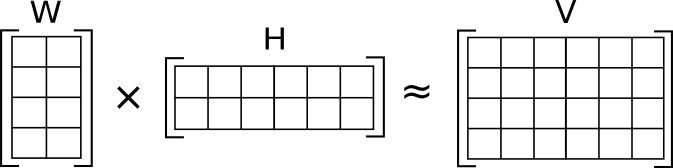
\includegraphics[width=8.5cm]{figures/NMF}}
%  \vspace{2.0cm}
  \medskip
\end{minipage}

\caption{Matrix $\mathbf{V}$ can be factorized into two matrices $\mathbf{W}$ and $\mathbf{H}$, so that their sum approximates $\mathbf{V}$. \scriptsize{\textsf{\textcopyright} WikiMedia CC BY-SA 3.0}}
\label{fig:NMF}

\end{figure}

In our case we use the magnitude spectrum of a song as the $\mathbf{V}$ matrix and decomposed it into two matrices.
The first one contains the magnitude spectra of the individual components we are interested in ($\mathbf{W}$) and the second one contains the time-varying gain of these components ($\mathbf{H}$), which tells us when each of the components for the first matrix is active.
For that reason the $\mathbf{W}$ matrix is usually called component matrix and $\mathbf{H}$ is usually called activation matrix.
Again the sum of both of these matrices makes up an approximation of the original spectrum \cite{smaragdis2003}.
A visual representation of that can be seen in figure \ref{fig:MatrixOverview} (d).

For our use case we were not interested in finding all the components and their activations.
We were rather interested in finding the corresponding activation of a specific component, like that of a base drum or a hi-hat.
This is also possible using NMF.
In order to do so, we specified $\mathbf{W}$ as the spectrum of a base drum (see figure \ref{fig:MatrixOverview} (b)) and $\mathbf{V}$ continued to be the spectrum of the whole song (see figure \ref{fig:MatrixOverview} (a)).
The NMF then solves for the matrix $\mathbf{H}$ (see figure \ref{fig:MatrixOverview} (c)) which tells us at what point in time the specified base drum spectrum appears in the song.
In that setup the NMF essentially works as a pattern matching algorithm.

\begin{figure}[htb]

\begin{minipage}[b]{1.0\linewidth}
  \centering
  \centerline{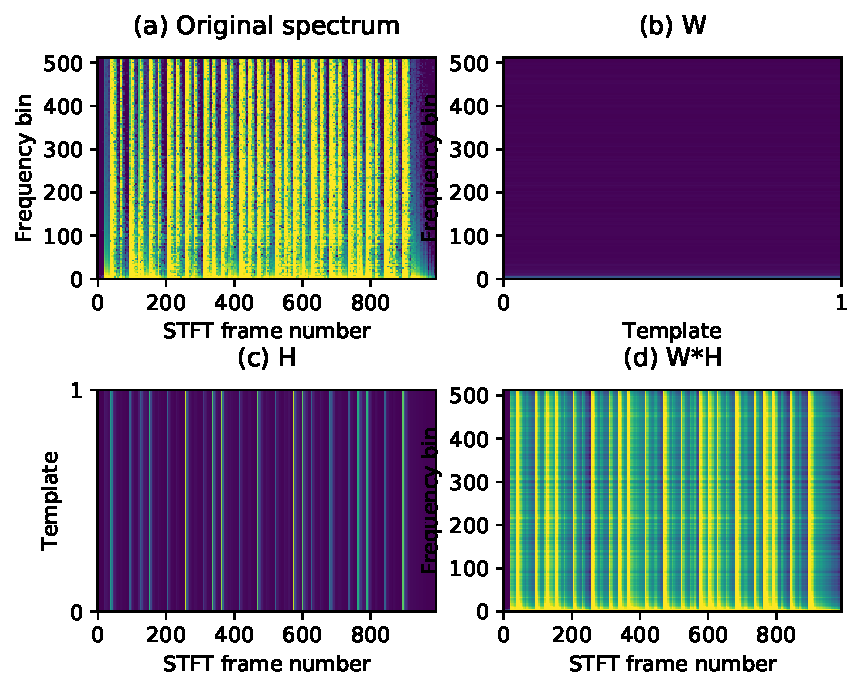
\includegraphics[width=8.5cm]{figures/MatrixOverview}}
%  \vspace{2.0cm}
  \medskip
\end{minipage}

\caption{(a) Magnitude spectrum of a drum track. (b) Magnitude spectrum of a base drum. (c) Activation matrix of the base drum. (d) Approximated spectrum. \scriptsize{\textsf{\textcopyright} Own work CC BY-SA 3.0}}
\label{fig:MatrixOverview}

\end{figure}


\begin{figure}[htb]

\begin{minipage}[b]{1.0\linewidth}
  \centering
  \centerline{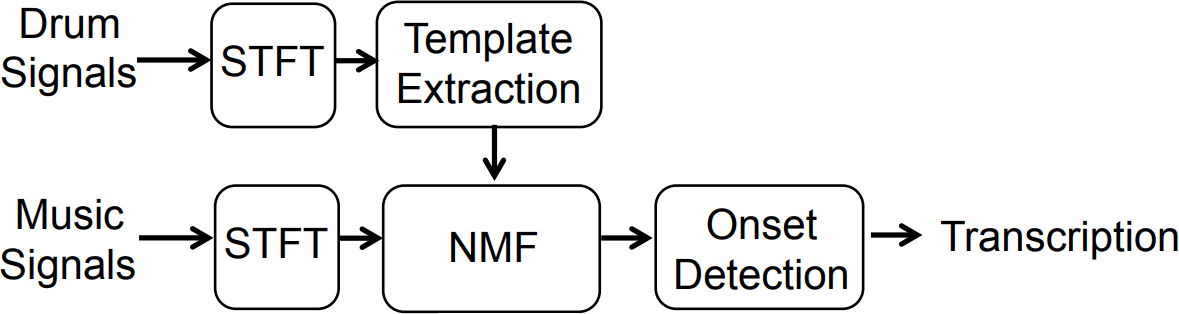
\includegraphics[width=8.5cm]{figures/Flowchart}}
%  \vspace{2.0cm}
  \medskip
\end{minipage}

\caption{Flowchart of the whole drum transcription algorithm. \scriptsize{\textsf{\textcopyright} Own work CC BY-SA 3.0}}
\label{fig:Flowchart}

\end{figure}


Figure \ref{fig:Flowchart} shows a flowchart with the complete overview of the algorithm we developed.
On the left hand side the two inputs to the algorithms are shown.
The first input is a time domain signal of percussive instrument, like a base drum or hi-hat, and the second input is a time domain signal of a piece of music.
For both inputs the first step is to down mix the signals into a mono signal.
Next the short-time Fourier transform (STFT) is applied, which transforms both signal from the time domain to the frequency domain.
For the parameters of the STFT we used a frame size of 1024 samples which yields in a frequency resolution of approx. 43 Hz per bin.
We also chose an overlap of 50\% between hops to improve the time resolution.
As mentioned before a visual representations of both transformed inputs can be found in figure \ref{fig:MatrixOverview} (b) and (a) respectively.

Before both inputs are fed into the actual detection the drum sound undergoes some further processing.
This step is marked as \textbf{template extraction} in figure \ref{fig:Flowchart}.
For our base drum template we chose to only use the transient of the base drum.
This has the advantage that it makes the template independent of the length of the original base drum sound.
As most of the energy is in the transient it is the most relevant part of the base drum sound.
Using only the transient also makes the template somewhat independent of the room it was recorded in, as any possible reverberation or echo is cut off.


After both inputs are prepared they are handed over to the NMF, which does its processing in the way described before.
The result of the NMF is in our case the activation matrix $\mathbf{H}$.
The matrix $\mathbf{H}$ can also be viewed as a function curve of how much the given template is contributing to the given music signal over time.
The next step of the algorithm is called \textbf{onset detection} where we extract the exact time points from the matrix $\mathbf{H}$.
An alternative representation of the matrix $\mathbf{H}$ as a curve can be seen in figure \ref{fig:ActivationMatrix}.
\begin{figure}[htb]

\begin{minipage}[b]{1.0\linewidth}
  \centering
  \centerline{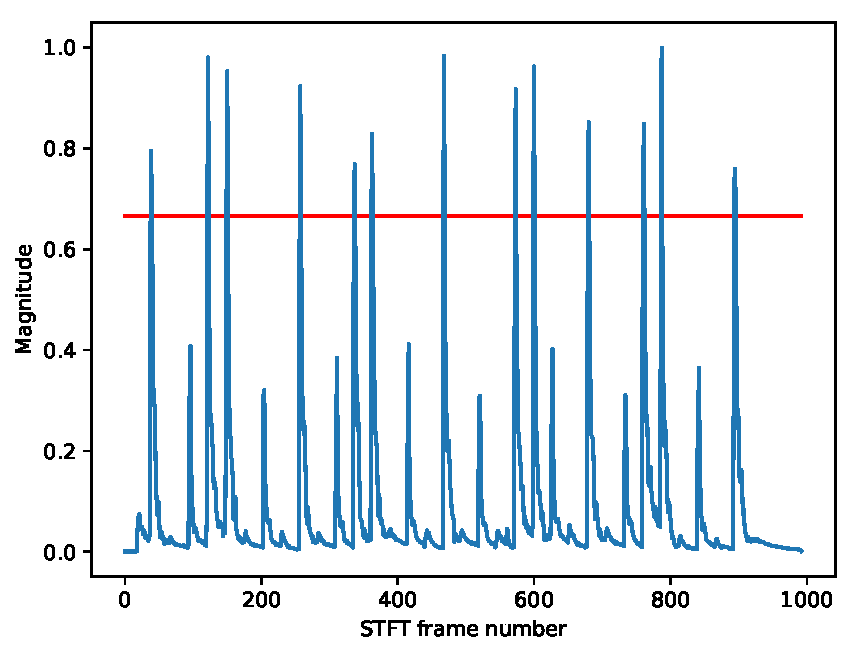
\includegraphics[width=6.7cm]{figures/ActivationMatrix}}
%  \vspace{2.0cm}
  \medskip
\end{minipage}

\caption{Example of the representation of an activation matrix as a curve. With a red line marking the threshold at $\frac{2}{3}$. \scriptsize{\textsf{\textcopyright} Own work CC BY-SA 3.0}}
\label{fig:ActivationMatrix}

\end{figure}
The onset detection is a simple implementation loosely based on the algorithms described by Lerch \cite{lerch2012book} in chapter 6.3.
To extract the onsets of the drum events the significant local maxima of the curve (peaks) have to be detected.
In order to do that the curve is first normalized.
Afterwards a threshold of $\frac{2}{3}$ is applied, which can be seen as a red line in figure \ref{fig:ActivationMatrix}.
This value was establish empirically to separate the valid detections from false positives.
Then the first derivative, which represents the slope of the curve, is calculated, by subtracting each element from the previous one.
An example of the resulting curve can be found in figure \ref{fig:Ableitung}.
In order to find the extract time points of a peak the zero crossings of the resulting curve have to be detected.
Once the frame number of a zero crossing is found, the frame number has to be converted back to a time point.
This is achieved by applying the following formula, where $f_s$ is the sample rate.

\begin{align}
\label{eq:timePoint}
timePoint = zeroCrossingFrameNumber * \frac{hopSize}{f_s}
\end{align}

Due to the formula \ref{eq:timePoint} we are only able to get the time point within a range of approx. 12 ms (called epsilon).
Once this calculation is done we receive a list of time points where the given template is found in the song which is the drum transcription we were looking for.

\begin{figure}[htb]

\begin{minipage}[b]{1.0\linewidth}
  \centering
  \centerline{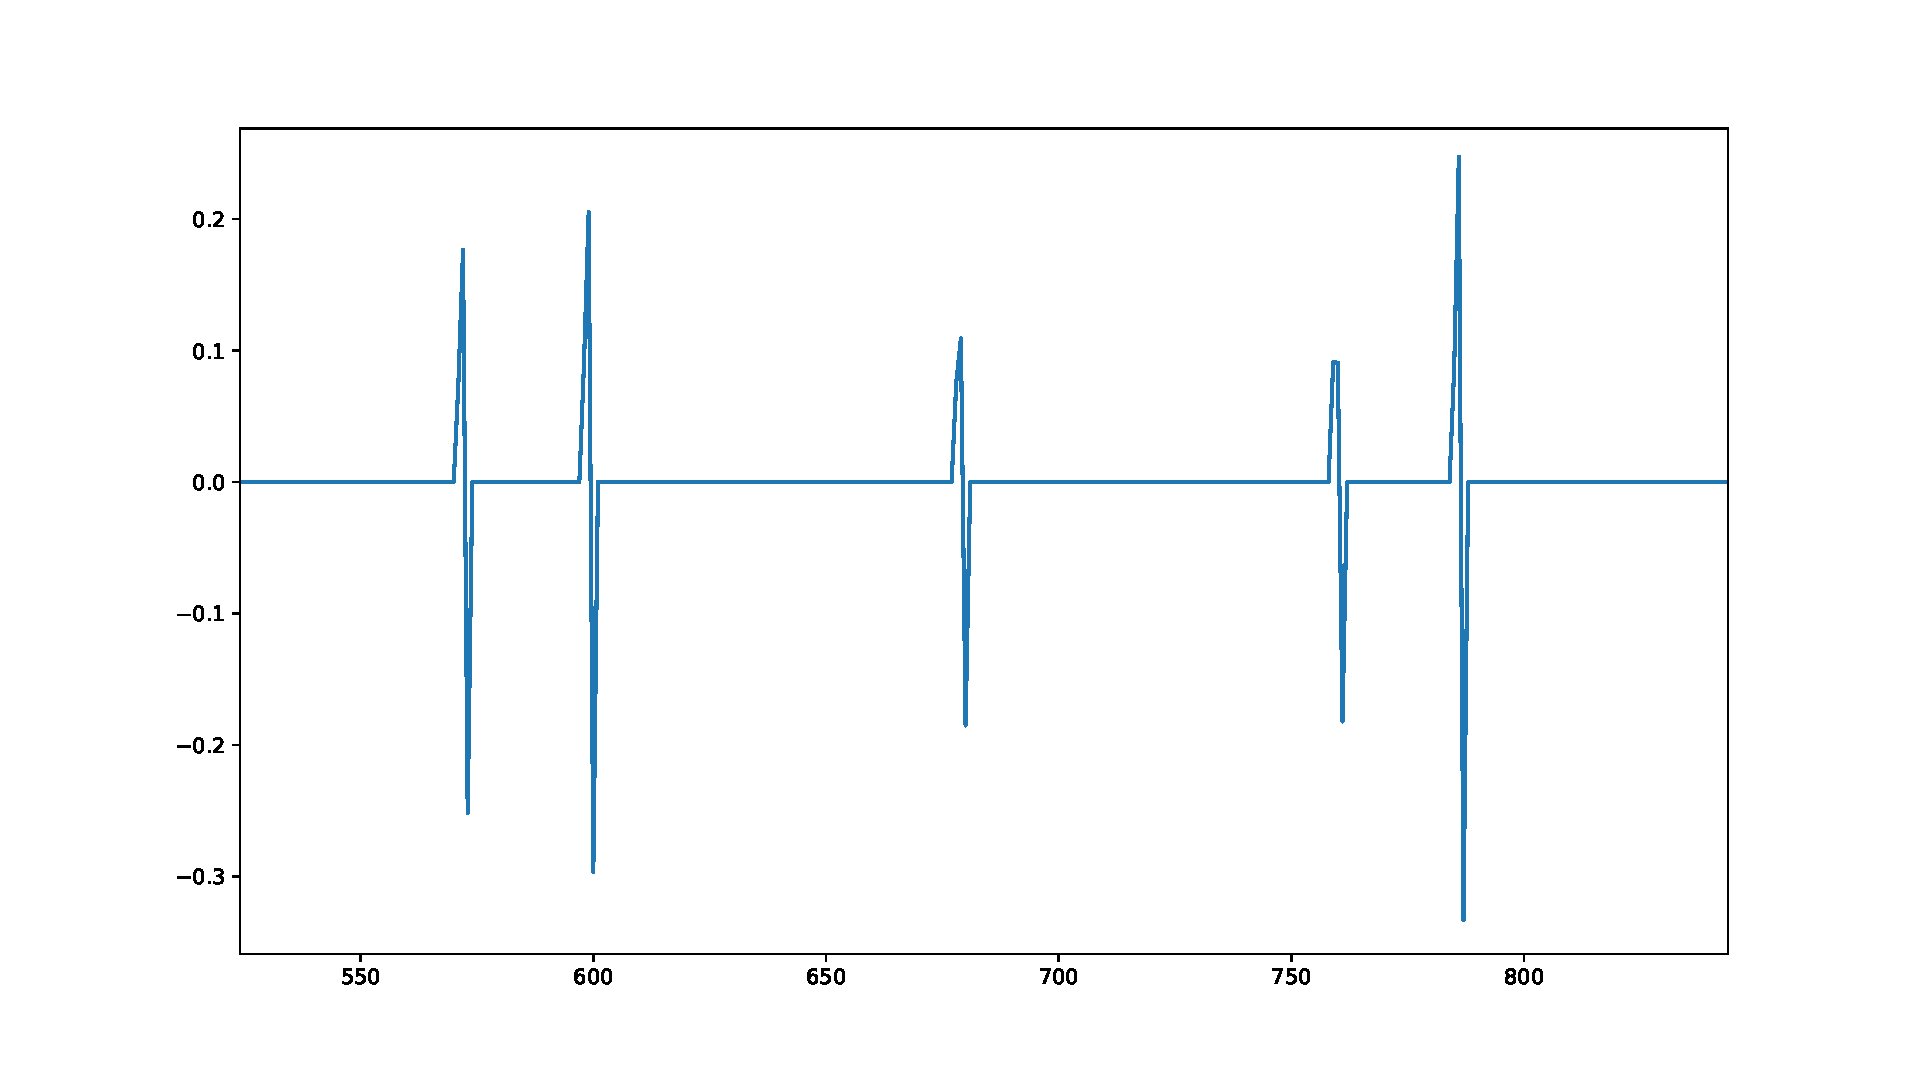
\includegraphics[width=8.5cm]{figures/Ableitung}}
%  \vspace{2.0cm}
  \medskip
\end{minipage}

\caption{An example of the first derivative of the activation function. \scriptsize{\textsf{\textcopyright} Own work CC BY-SA 3.0}}
\label{fig:Ableitung}

\end{figure}


The implementation of our algorithm was done in Python using the numpy/scipy library stack. 
As well as the library nimfa\footnote{\url{http://nimfa.biolab.si/}} for NMF calculations.
The entire code repository is licensed under the GPL 3.0 and can be found on GitHub\footnote{\url{https://github.com/Bendrien/AudioContentAnalysis}}.

%basic NMF description, our peak picking algorithm, maybe libs used

% section algo (end)


\section{Evaluation}
\label{sec:evaluation}

As our test data set we used the ENST-drums database of the Institut Télécom Paris Tech\footnote{\url{https://perso.telecom-paristech.fr/~grichard/ENST-drums/}}.
The data set contains recordings of 207 drum tracks split over 3 different drum kits.
In the data set each instrument of the drum kit is recorded separately.
For our purposes we only uses the mixed version of the tracks called ``wet-mix'' which also contains some acoustic elements of the recording room, like reverberation, making it more realistic for real world applications.
Next to the recordings the test data set also contains a annotation file for each drum track, which lists the occurrence an instrument as well as the time point it occurred.
This data was used as the ground truth to compare our algorithm against.

In order to evaluate the accuracy of our algorithm we compared the drum events that our algorithm detected with the annotations of the ENST test set.
When comparing the results we took into account the epsilon error margin of approx. 12 ms.


  \begin{table}[h]
    \centering
    \begin{tabular}{l | c c c}
      Drummer  &  1 & 2 & 3 \\
      \# Files &   63 &   75 & 69 \\
      \hline
      Median$_{P}$   & 0.25 & 0.93 & 0.86 \\
      Mean$_{P}$     & 0.27 & 0.89 & 0.80 \\
      $\sigma_P$     & 0.22 & 0.12 & 0.18 \\
      \hline
      Median$_{FP}$   & 0.13 & 0.0 & 0.0 \\
      Mean$_{FP}$     & 0.23 & 0.0 & 0.001 \\
      $\sigma_{FP}$   & 0.29 & 0.0 & 0.001 \\
    \end{tabular}
    \caption{Results of the base drum detection. $P$ represents the true positives and $FP$ the false positives.}
    \label{tab:results}
  \end{table}

ground truth, methodology, metrics
results
discussion

- we only uses drum tracks, but it also works with mixed music. problem: ground truth

% section evaluation (end)


\section{Conclusion}
\label{sec:conclusion}

summary, noteworthy parts of the presented work,
achievements and contributions
possible improvements and future work

Improvements: 
- Using adaptive templates like shown in \cite{lerch2015} can help the "over-fitting" of a template.
- adaptive threshold instead of 2/3
- sinc interpolation to reduce epsilon

% section conclusion (end)

% References should be produced using the bibtex program from suitable
% BiBTeX files (here: strings, refs, manuals). The IEEEbib.bst bibliography
% style file from IEEE produces unsorted bibliography list.
% -------------------------------------------------------------------------
\bibliographystyle{IEEEbib}
\bibliography{strings,refs}

%\end{document}


% DELETE EVERYTHING FROM HERE IN THE END
% DELETE EVERYTHING FROM HERE IN THE END
% DELETE EVERYTHING FROM HERE IN THE END

\vfill\pagebreak

\section{common flaws}
all cited papers should appear in bibliography
vice versa: all references should be mentioned in the paper
each reference should contain:
names of authors
title of the paper or book
conference paper: name of conf. incl. year and location
journal paper: name of journal incl. volume, year and pages
book: publisher, potentially editor
all figures and tables must be referenced in the paper
equations:
all mathematical symbols must be explained
symbols should be used consistently and unambiguously
abbreviations (STFT, DFT, etc.) should be introduced
”The short-time Fourier transform (STFT) is given by (. . .)
We compute the STFT of the signal, (. . .)”

\section{Evaluation}

form (structure, language, form of references)
content (introduction, literature review, algorithm and
evaluation description, figures, comprehensibility, correctness)
evaluation (dataset, metrics, discussion)

\vfill\pagebreak
~
\vfill\pagebreak


The abstract should appear at the top of the left-hand column of text, about
0.5 inch (12 mm) below the title area and no more than 3.125 inches (80 mm) in
length.  Leave a 0.5 inch (12 mm) space between the end of the abstract and the
beginning of the main text.  The abstract should contain about 100 to 150
words, and should be identical to the abstract text submitted electronically
along with the paper cover sheet.  All manuscripts must be in English, printed
in black ink.


These guidelines include complete descriptions of the fonts, spacing, and
related information for producing your proceedings manuscripts. Please follow
them and if you have any questions, direct them to Conference Management
Services, Inc.: Phone +1-979-846-6800 or email
to \\\texttt{papers@icassp2016.org}.

\section{Formatting your paper}
\label{sec:format}

All printed material, including text, illustrations, and charts, must be kept
within a print area of 7 inches (178 mm) wide by 9 inches (229 mm) high. Do
not write or print anything outside the print area. The top margin must be 1
inch (25 mm), except for the title page, and the left margin must be 0.75 inch
(19 mm).  All {\it text} must be in a two-column format. Columns are to be 3.39
inches (86 mm) wide, with a 0.24 inch (6 mm) space between them. Text must be
fully justified.

\section{PAGE TITLE SECTION}
\label{sec:pagestyle}

The paper title (on the first page) should begin 1.38 inches (35 mm) from the
top edge of the page, centered, completely capitalized, and in Times 14-point,
boldface type.  The authors' name(s) and affiliation(s) appear below the title
in capital and lower case letters.  Papers with multiple authors and
affiliations may require two or more lines for this information. Please note
that papers should not be submitted blind; include the authors' names on the
PDF.

\section{TYPE-STYLE AND FONTS}
\label{sec:typestyle}

To achieve the best rendering both in printed proceedings and electronic proceedings, we
strongly encourage you to use Times-Roman font.  In addition, this will give
the proceedings a more uniform look.  Use a font that is no smaller than nine
point type throughout the paper, including figure captions.

In nine point type font, capital letters are 2 mm high.  {\bf If you use the
smallest point size, there should be no more than 3.2 lines/cm (8 lines/inch)
vertically.}  This is a minimum spacing; 2.75 lines/cm (7 lines/inch) will make
the paper much more readable.  Larger type sizes require correspondingly larger
vertical spacing.  Please do not double-space your paper.  TrueType or
Postscript Type 1 fonts are preferred.

The first paragraph in each section should not be indented, but all the
following paragraphs within the section should be indented as these paragraphs
demonstrate.

\section{MAJOR HEADINGS}
\label{sec:majhead}

Major headings, for example, "1. Introduction", should appear in all capital
letters, bold face if possible, centered in the column, with one blank line
before, and one blank line after. Use a period (".") after the heading number,
not a colon.

\subsection{Subheadings}
\label{ssec:subhead}

Subheadings should appear in lower case (initial word capitalized) in
boldface.  They should start at the left margin on a separate line.
 
\subsubsection{Sub-subheadings}
\label{sssec:subsubhead}

Sub-subheadings, as in this paragraph, are discouraged. However, if you
must use them, they should appear in lower case (initial word
capitalized) and start at the left margin on a separate line, with paragraph
text beginning on the following line.  They should be in italics.

\section{PRINTING YOUR PAPER}
\label{sec:print}

Print your properly formatted text on high-quality, 8.5 x 11-inch white printer
paper. A4 paper is also acceptable, but please leave the extra 0.5 inch (12 mm)
empty at the BOTTOM of the page and follow the top and left margins as
specified.  If the last page of your paper is only partially filled, arrange
the columns so that they are evenly balanced if possible, rather than having
one long column.

In LaTeX, to start a new column (but not a new page) and help balance the
last-page column lengths, you can use the command ``$\backslash$pagebreak'' as
demonstrated on this page (see the LaTeX source below).

\section{PAGE NUMBERING}
\label{sec:page}

Please do {\bf not} paginate your paper.  Page numbers, session numbers, and
conference identification will be inserted when the paper is included in the
proceedings.

\section{ILLUSTRATIONS, GRAPHS, AND PHOTOGRAPHS}
\label{sec:illust}

Illustrations must appear within the designated margins.  They may span the two
columns.  If possible, position illustrations at the top of columns, rather
than in the middle or at the bottom.  Caption and number every illustration.
All halftone illustrations must be clear black and white prints.  Colors may be
used, but they should be selected so as to be readable when printed on a
black-only printer.

Since there are many ways, often incompatible, of including images (e.g., with
experimental results) in a LaTeX document, below is an example of how to do
this.

\section{FOOTNOTES}
\label{sec:foot}

Use footnotes sparingly (or not at all!) and place them at the bottom of the
column on the page on which they are referenced. Use Times 9-point type,
single-spaced. To help your readers, avoid using footnotes altogether and
include necessary peripheral observations in the text (within parentheses, if
you prefer, as in this sentence).

% Below is an example of how to insert images. Delete the ``\vspace'' line,
% uncomment the preceding line ``\centerline...'' and replace ``imageX.ps''
% with a suitable PostScript file name.
% -------------------------------------------------------------------------
\begin{figure}[htb]

\begin{minipage}[b]{1.0\linewidth}
  \centering
  \centerline{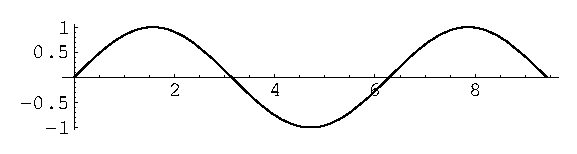
\includegraphics[width=8.5cm]{figures/image1}}
%  \vspace{2.0cm}
  \centerline{(a) Result 1}\medskip
\end{minipage}
%
\begin{minipage}[b]{.48\linewidth}
  \centering
  \centerline{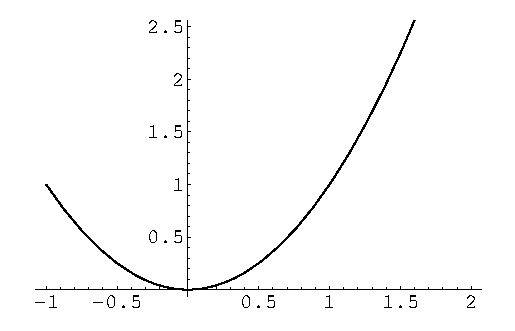
\includegraphics[width=4.0cm]{figures/image3}}
%  \vspace{1.5cm}
  \centerline{(b) Results 3}\medskip
\end{minipage}
\hfill
\begin{minipage}[b]{0.48\linewidth}
  \centering
  \centerline{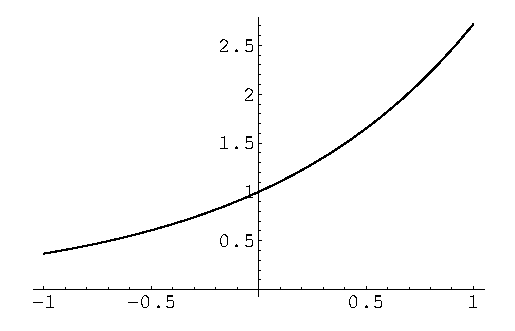
\includegraphics[width=4.0cm]{figures/image4}}
%  \vspace{1.5cm}
  \centerline{(c) Result 4}\medskip
\end{minipage}
%
\caption{Example of placing a figure with experimental results.}
\label{fig:res}
%
\end{figure}


% To start a new column (but not a new page) and help balance the last-page
% column length use \vfill\pagebreak.
% -------------------------------------------------------------------------
%\vfill
%\pagebreak

\section{COPYRIGHT FORMS}
\label{sec:copyright}

You must submit your fully completed, signed IEEE electronic copyright release
form when you submit your paper. We {\bf must} have this form before your paper
can be published in the proceedings.

\section{RELATION TO PRIOR WORK}
\label{sec:prior}

The text of the paper should contain discussions on how the paper's
contributions are related to prior work in the field. It is important
to put new work in  context, to give credit to foundational work, and
to provide details associated with the previous work that have appeared
in the literature. This discussion may be a separate, numbered section
or it may appear elsewhere in the body of the manuscript, but it must
be present.

You should differentiate what is new and how your work expands on
or takes a different path from the prior studies. An example might
read something to the effect: "The work presented here has focused
on the formulation of the ABC algorithm, which takes advantage of
non-uniform time-frequency domain analysis of data. The work by
Smith and Cohen considers only fixed time-domain analysis and
the work by Jones et al takes a different approach based on
fixed frequency partitioning. While the present study is related
to recent approaches in time-frequency analysis [3-5], it capitalizes
on a new feature space, which was not considered in these earlier
studies."

\vfill\pagebreak

\section{REFERENCES}
\label{sec:refs}

List and number all bibliographical references at the end of the
paper. The references can be numbered in alphabetic order or in
order of appearance in the document. When referring to them in
the text, type the corresponding reference number in square
brackets as shown at the end of this sentence. An
additional final page (the fifth page, in most cases) is
allowed, but must contain only references to the prior
literature.

\end{document}
